\graphicspath{{results/fig/}}

\chapter{Practical implementation and results}
\label{chap:results}

    \paragraph
    In previous chapters, it was shown with simulation data that both the white-box and black-box system identification models can
    accurately represent the dynamics of a multirotor with a suspended payload.
    However, practical flights may differ significantly from simulations, which would affect the performance of these techniques.
    Wind is a common cause of unmeasured disturbances that influences the flight of a multirotor, 
    but this disturbance was not considered in simulations.
    The practical dynamics and sensor noise may also differ from the simulation model, which further motivates the need for practical data.
    
    \paragraph
    In this chapter, the system identification techniques will be applied to practical flight data.
    The effect of different system configurations and wind conditions on the performance of these techniques will be investigated.
    These techniques will also be applied and evaluated with a practical dynamic payload.
    % Furthermore, the suitability of the system identification models
    % for swing damping control will be investigated in simulations.
    % The performance of the swing damping controllers will be evaluated for a range of different system configurations.
    HITL simulations will also be performed to determine whether the proposed hardware can handle the computational complexity of these algorithms.
    Finally, the practical feasibility of the proposed system identification and control architectures will be discussed.
    
    \FloatBarrier\section{Methodology}
        
        \paragraph
        As discussed in Chapter~\ref{chap:system_id}, 
        generating data for the parameter estimation techniques involves two distinct flight stages.
        Firstly, the multirotor hovers with the suspended payload to gather data for payload mass estimation.
        A velocity step setpoint is then commanded to stimulate the swinging payload system for cable length estimation.
        Hence, the same methodology used for simulations will be used for practical flights.

        \paragraph
        For the data-driven techniques, the generation of practical training and testing data
        also follows the same general methodology as simulated flights:
        \begin{enumerate}
            \item Data logging starts when the multirotor is armed
            \item Takeoff and hover with the multirotor
            \item Command velocity step setpoints
            \item Land the multirotor
            \item Data logging stops when the multirotor is disarmed
            \item Download the data log from the multirotor
            \item Split the data into separate training and testing periods
            \item Build a model from the training data
            \item Perform model predictions over the testing data to calculate an error metric
        \end{enumerate}

        \paragraph
        Figure~\ref{fig:honeybee_with_payload} shows the Honeybee multirotor with a suspended payload during a practical flight.
        Numerous flights were performed with different 
        payload masses, 
        cable lengths, 
        wind conditions, 
        and dynamic payloads.
        The system identification methods were then performed on data resulting from this wide range of different use cases.
        
        \paragraph
        The major differences between the simulated and practical flights involve the attachment of the payload and wind disturbances.
        In simulations, the payload cable is attached to the exact \gls{CoM} of the multirotor.
        However, for practical flights the cable is attached slightly below the \gls{CoM} of Honeybee due to mechanical constraints.
        Practical flights are also influenced by wind disturbances which were not considered in simulations.
        The measurement noise experienced by a practical multirotor may also differ from the noise models used in simulations.
        Therefore this effect will also be investigated in the sections below.

        \begin{figure}[!htb]
            \centering
            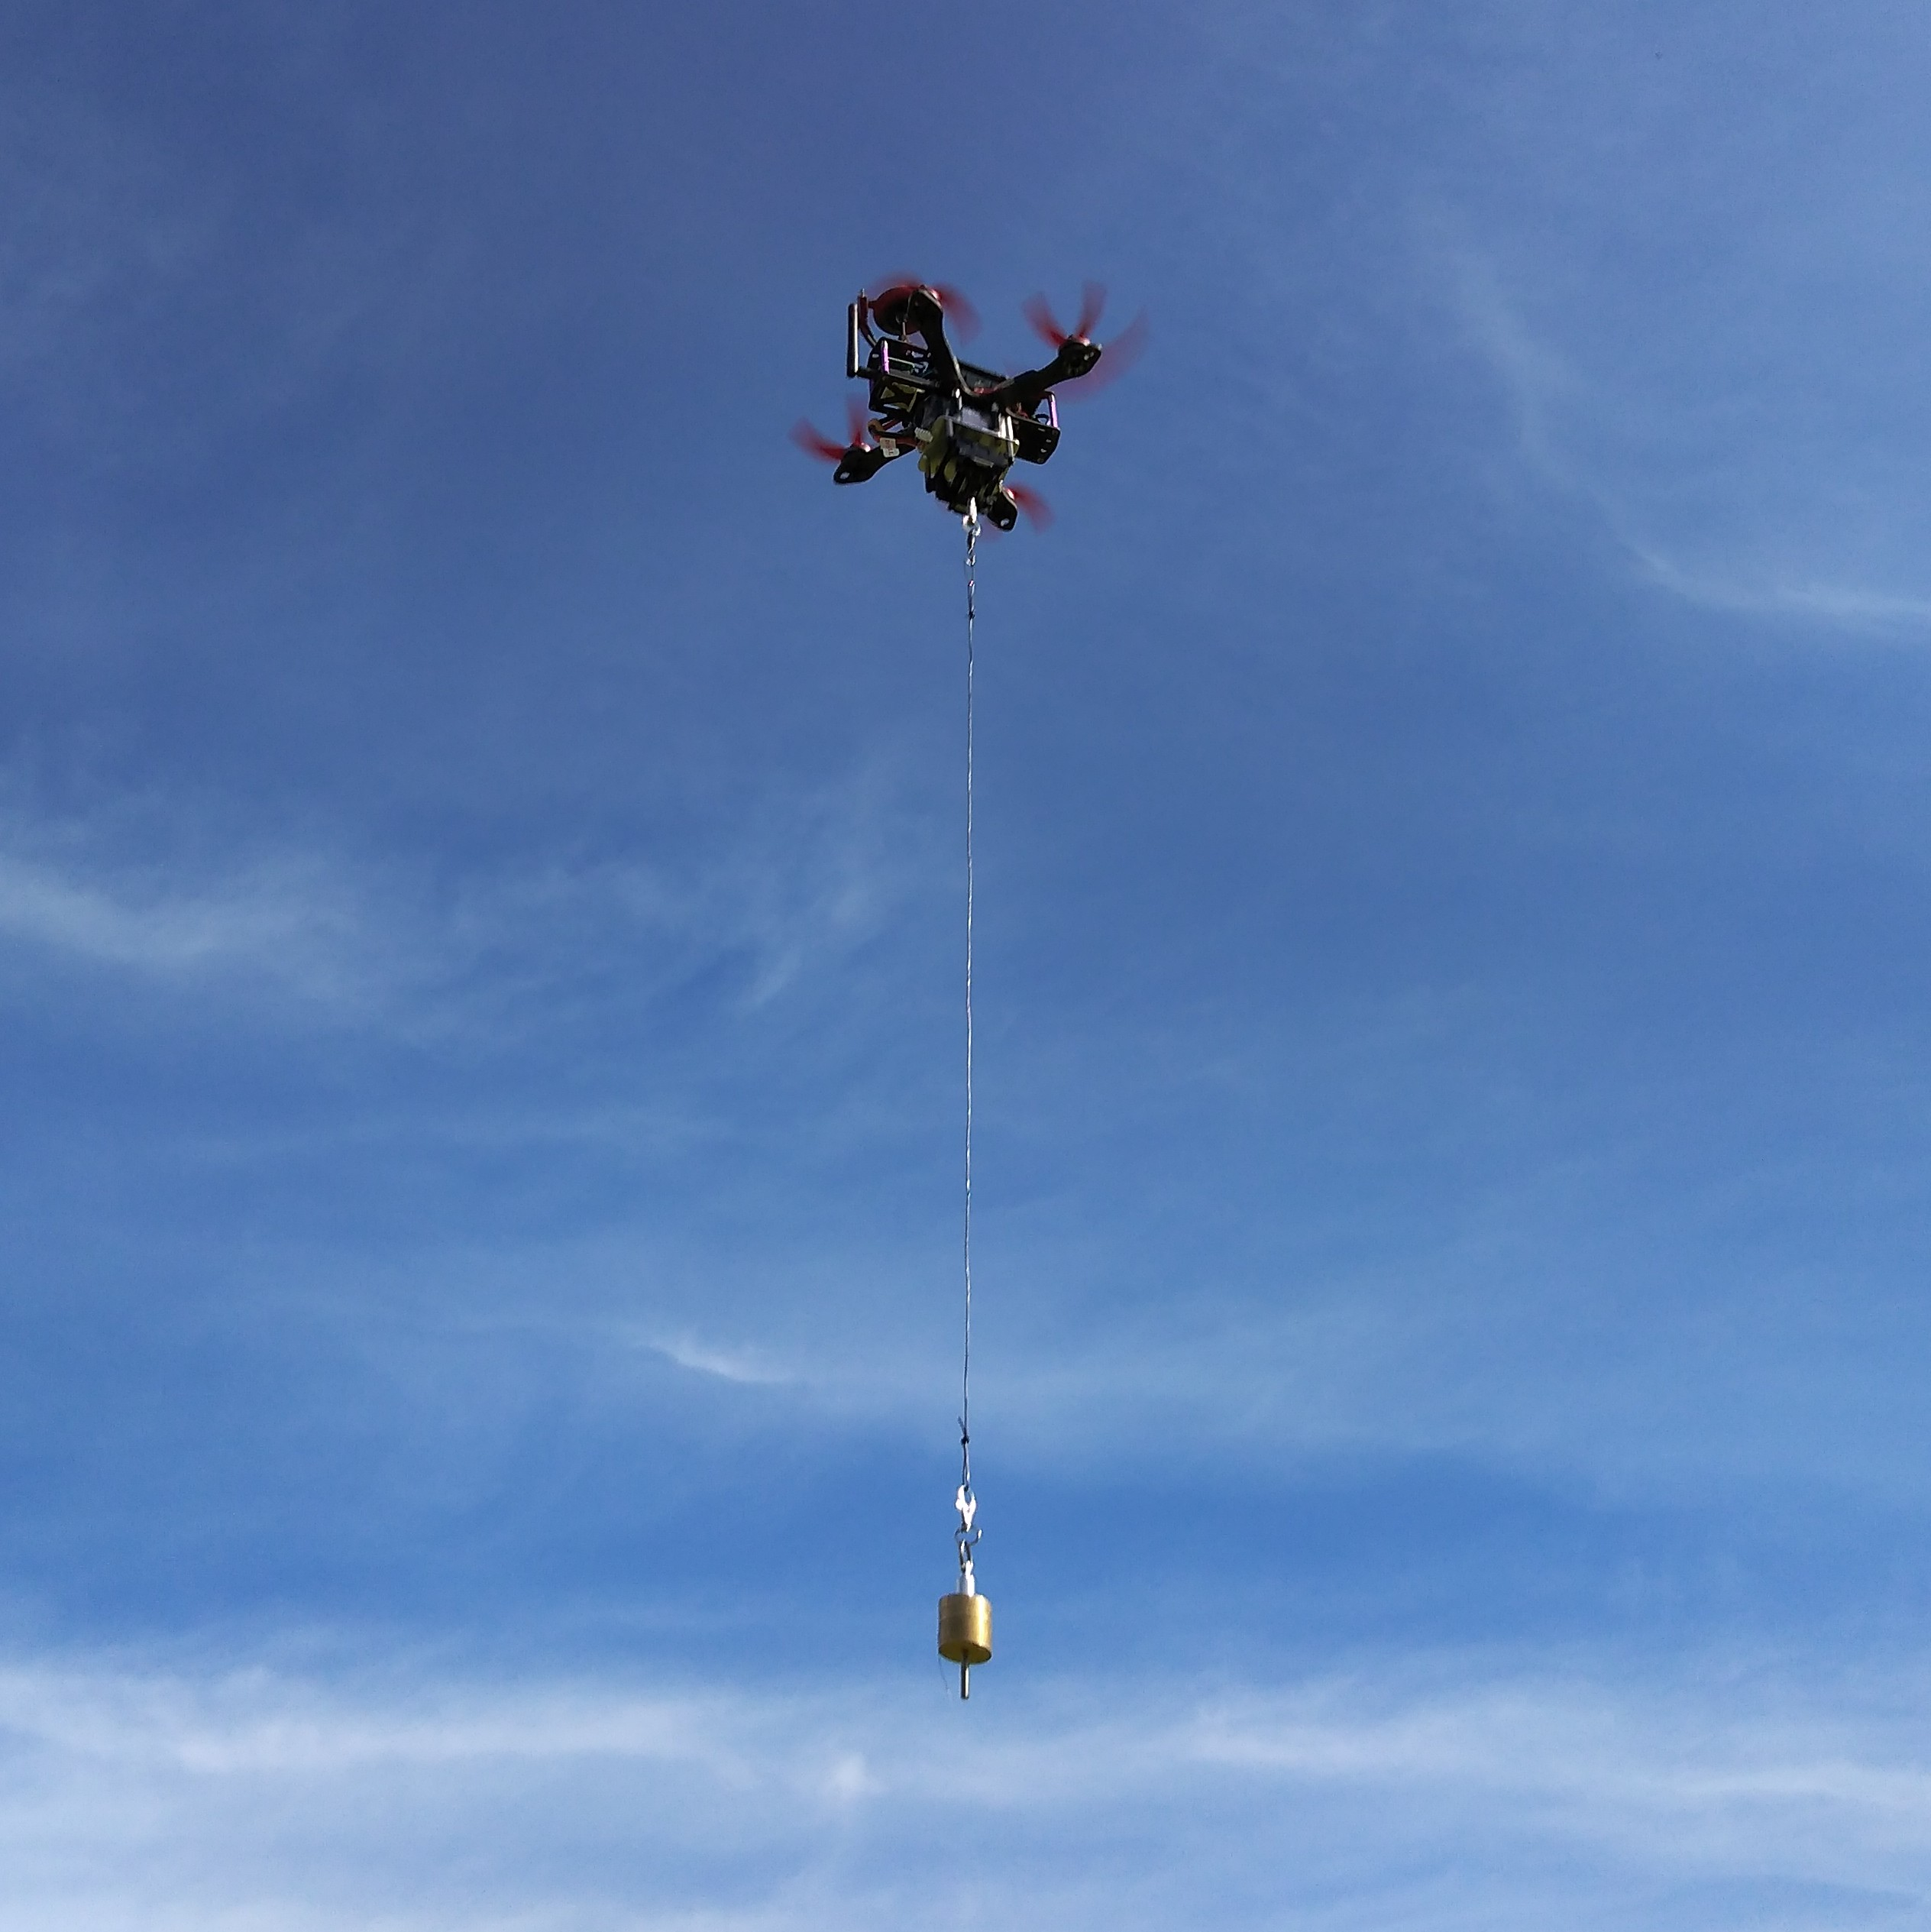
\includegraphics[width=0.5\linewidth]{honeybee_with_payload.jpg}
            \caption{Practical flight with Honeybee and a suspended payload}
            \label{fig:honeybee_with_payload}
        \end{figure}
        
        % \begin{itemize}
        %     \item Method for generating data
        %     \item Plot example of training data
        %     \item picture of practical flight single and double
        %     \item Discuss difference between \gls{SITL} and prac
        %     \begin{itemize}
        %         \item Noise 
        %         \item wind
        %         \item \gls{CoM}
        %     \end{itemize}
        %     \item plot hover of prac vs \gls{SITL} to show noise and disturbance
        % \end{itemize}

        % \paragraph
        % In Chapter~\ref{chap:system_id} it was noted that the optimal length of training data 
        % often only included 2 velocity steps responses.
        % This means the models were trained on a very small sample of step sizes 
        % and need to extrapolate the dynamics of other step sizes.
        
    \FloatBarrier\section{Parameter estimation with practical data}

        \paragraph
        In Section~\ref{sec:param_estimation}, parameter estimation was performed with simulation data.
        It was shown that the models with the estimated parameter values provide reasonably accurate representations of the simulated dynamics.
        In this section, practical flight data will be used for parameter estimation.
        The effect of wind on the parameter estimation techniques will also be investigated.
        
        %% ?? Add this if there is time
        % \subsection{Mass estimation} 
        
        %     As discussed in Chapter~\ref{chap:system_id}, for this method to work, the mass of the multirotor needs to be known.
        %     If a heavier battery or an extra accessory is added to the vehicle, 
        %     the new vehicle mass will first have to be estimated in a separate flight, before the payload can be attached.
        %     This is one of the disadvantages of white-box modelling with parameter estimation based techniques.
        %     The method is designed with a specific system in mind 
        %     and needs to be adjusted and redesigned for every deviation from the the pre-assumed configuration.
        %     In contrast, the data-driven technique is a general solution which works for a much wider range of system configurations.
        %     The data-driven technique is not readjusted for an added vehicle mass, 
        %     since the whole model is estimated instead of specific parameters.

        \FloatBarrier\subsection{Simple payload cable length estimation}
            
            \paragraph
            As discussed in Section~\ref{sec:length_estimation}, an \gls{FFT} of the payload angle data is used to estimate the natural frequency of the suspended payload, 
            which is used to estimate the cable length.
            \gls{PE} will be used as the error metric to quantify the estimation accuracy.
            The \gls{PE} of the cable length estimation is calculated as,
            \begin{equation}
                PE = \frac{ l_{estimated} - l_{actual} }{ l_{actual} } \times 100 \% ,
            \end{equation}
            where $l_{actual}$ is the actual cable length and $l_{estimated}$ is the estimated cable length.
            The \gls{PE} can be interpretted as the percentage of the actual length by which the estimated length differs from the actual length.
            
            \begin{figure}[htb]
    \centering
    \begin{tikzpicture}
        \begin{axis}[            
            xlabel = Length of training data,
            ylabel = Estimated cable length,
            x unit = \si{\second},
            y unit = \%,
            xmin = 0,   xmax = 15,
            ymin = -50,   ymax = 150,
            grid = major,
            legend cell align = left,
            legend pos = north east,
            grid style = dashed,
            legend style = {font = \scriptsize},
            label style = {font = \scriptsize},
            tick label style = {font = \scriptsize},
            width = 0.95\columnwidth,
            height = 0.5\columnwidth,
            % initialize Dark2
            cycle list/Dark2,
            % combine it with 'mark list*':
            cycle multiindex* list = {
                Dark2\nextlist
            }
        ]

        \addplot+[mark = none, style = solid, ultra thick] 
        table[x = train_time, y = percentage_error, col sep = comma] 
        {results/csv/cable_length_vs_train_time_Prac_2021-08-23_01_l-0.5_mp-0.2_wind-0.5.csv_10_0.5.csv};
        \addlegendentry{$m_p =$~\SI{0.2}{\kilo\gram}, $l =$~\SI{0.5}{\meter}}

        \addplot+[mark = none, style = solid, ultra thick] 
        table[x = train_time, y = percentage_error, col sep = comma] 
        {results/csv/cable_length_vs_train_time_Prac_2021-08-20_01_l-1_mp-0.1_wind-0.5.csv_10_1.csv};
        \addlegendentry{$m_p =$~\SI{0.1}{\kilo\gram}, $l =$~\SI{1}{\meter}}        

        \addplot+[mark = none, style = solid, ultra thick] 
        table[x = train_time, y = percentage_error, col sep = comma] 
        {results/csv/cable_length_vs_train_time_Prac_2021-08-20_02_l-2_mp-0.3-wind-0.5.csv_10_2.csv};
        \addlegendentry{$m_p =$~\SI{0.3}{\kilo\gram}, $l =$~\SI{2}{\meter}}

        \addplot+[mark = none, style = solid, ultra thick] 
        table[x = train_time, y = percentage_error, col sep = comma] 
        {results/csv/cable_length_vs_train_time_Prac_2021-08-20_03_l-1_mp-0.2_wind-0.5.csv_10_1.csv};
        \addlegendentry{$m_p =$~\SI{0.2}{\kilo\gram}, $l =$~\SI{1}{\meter}}
        
        \end{axis}
    \end{tikzpicture} 
    
    \caption{}
    \label{fig:cable_length_vs_train_time}
\end{figure}


            \paragraph
            Figure~\ref{fig:cable_length_vs_train_time} shows the \gls{PE} of the cable length estimation 
            with different payload masses and cable lengths.
            Note that for each payload configuration, 
            the estimation converges to a constant error after a sufficient length of training data.
            %% ?? Add length of training data required to all techniques to compare white-box length to black box length
            For these payload configurations, the converged \gls{PE} ranges from 18.9~\% to 32.4~\%.
            These errors may be due to the large difference between the theoretical and the damped natural frequency.
            It appears that the \gls{PID} controllers damp the payload oscillations significantly, 
            which affects the oscillation frequency of the payload.
            Hence, an incorrect length is estimated from the frequency peak identified in the \gls{FFT}.
            
            \begin{figure}[htb]
    \centering
    \begin{tikzpicture}
        \begin{axis}[            
            xlabel = Time,
            ylabel = Payload angle,
            x unit = \si{\second},
            y unit = \si{\radian},
            xmin = 0,   xmax = 20,
            ymin = -20,  ymax = 20,
            grid = major,
            legend cell align = left,
            legend pos = north east,
            grid style = dashed,
            legend style = {font = \scriptsize},
            label style = {font = \scriptsize},
            tick label style = {font = \scriptsize},
            width = 0.95\columnwidth,
            height = 0.5\columnwidth,
            % initialize Dark2
            cycle list/Dark2,
            % combine it with 'mark list*':
            cycle multiindex* list = {
                Dark2\nextlist
            }
        ]
        
        \addplot+[mark = none, style = solid, ultra thick] 
        table[x = time, y = theta, col sep = comma] 
        {results/csv/step_predictions_Prac_2021-08-20_02_l-2_mp-0.3-wind-0.5.csv_white_26.34.csv};
        \addlegendentry{Actual}

        \addplot+[mark = none, style = solid, ultra thick] 
        table[x = time, y = theta_hat, col sep = comma] 
        {results/csv/step_predictions_Prac_2021-08-20_02_l-2_mp-0.3-wind-0.5.csv_white_26.34.csv};
        \addlegendentry{Model prediction using the estimated length}

        \end{axis}
    \end{tikzpicture} 
    
    \caption{White-box model prediction for a North velocity step input
    ($l =$~\SI{0.5}{\metre}, $m_p =$~\SI{0.2}{\kilo\gram}.)}
    \label{fig:prediction_single_pend_white_prac}
\end{figure}


            \paragraph
            Figure~\ref{fig:prediction_single_pend_white_prac} compares the actual payload angle to the predicted angle of the white-box model for a practical flight. 
            The cable length estimated from this flight is \SI{0.617}{\metre} resulting in a \gls{PE} of 23.4~\%.
            It is clear that the prediction differs significantly from the actual data in magnitude and in frequency.
            A large difference is expected at such large swing angles, because the model was a linearised with the small angle approximation (as discussed in Chapter~\ref{chap:modelling}).
            Therefore, the actual non-linear dynamics differ significantly from the linearised model for this data.
            Note that an incorrect damping coefficient used in the model does can not contribute much to the modelling error.
            The damping coefficient largely effects the rate of attenuation of the amplitude of the oscillations, but does not have a large effect on the initial swing angle of the predicted by the model.
            The initial swing angle of the practical data is clearly very different from the model prediction.
            
            \begin{figure}[htb]
    \centering
    \begin{tikzpicture}
        \begin{axis}[            
            xlabel = Time,
            ylabel = Payload angle,
            x unit = \si{\second},
            y unit = \si{\degree},
            xmin = 0,   xmax = 20,
            ymin = -20,  ymax = 20,
            grid = major,
            legend cell align = left,
            legend pos = north east,
            grid style = dashed,
            legend style = {font = \scriptsize},
            label style = {font = \scriptsize},
            tick label style = {font = \scriptsize},
            width = 0.95\columnwidth,
            height = 0.5\columnwidth,
            % initialize Dark2
            cycle list/Dark2,
            % combine it with 'mark list*':
            cycle multiindex* list = {
                Dark2\nextlist
            }
        ]
        
        \addplot+[mark = none, style = solid, ultra thick] 
        table[x = time, y = theta, col sep = comma] 
        {results/csv/step_predictions_Prac_2021-08-20_02_l-2_mp-0.3-wind-0.5.csv_white_21.74.csv};
        \addlegendentry{Actual}

        \addplot+[mark = none, style = solid, ultra thick] 
        table[x = time, y = theta_hat, col sep = comma] 
        {results/csv/step_predictions_Prac_2021-08-20_02_l-2_mp-0.3-wind-0.5.csv_white_21.74.csv};
        \addlegendentry{Model prediction using the estimated length}

        \end{axis}
    \end{tikzpicture} 
    
    \caption{White-box model prediction for a North velocity step input
    ($l =$~\SI{0.5}{\metre}, $m_p =$~\SI{0.2}{\kilo\gram}.).}
    \label{fig:prediction_single_pend_white_prac_bad}
\end{figure}


            \paragraph
            The naive assumption regarding the speed of the inner loop \gls{PID} controller probably adds to the modelling error significantly.
            As discussed in Chapter~\ref{chap:modelling}, the white-box model assumes that the time scale seperation between the velocity and attitude controller is large enough for the acceleration setpoint to approximate the actual seperation.
            However, it appears that the attitude controller of the practical multirotor is slow enough to significantly affect the transient response of the swing angle.
            Notice how the first two oscillation peaks differ noticeably from the expected linear damping shape.
            Since the payload is attached below the \gls{CoM} of the multirotor, the oscillating pitch angle of the multirotor also affects the swing angle of the payload.

            % ?? However, as discussed in Chapter~\ref{chap:control_systems}, the LQR controller which utillises the white-box model is quite robust against model uncertainty and may still result in acceptable control with such a model.
            % Recall from Chapter~\ref{chap:system_id} that the damping coefficient is not estimated, but a manually tuned value is used.

            \begin{figure}[htb]
    \centering
    \begin{tikzpicture}
        \begin{axis}[            
            xlabel = Length of training data,
            ylabel = Percentage Error,
            x unit = \si{\second},
            y unit = \%,
            xmin = 0,       xmax = 12,
            ymin = -50,     ymax = 100,
            grid = major,
            legend cell align = left,
            legend pos = north east,
            grid style = dashed,
            legend style = {font = \scriptsize},
            label style = {font = \scriptsize},
            tick label style = {font = \scriptsize},
            width = 0.95\columnwidth,
            height = 0.5\columnwidth,
            % initialize Dark2
            cycle list/Dark2,
            % combine it with 'mark list*':
            cycle multiindex* list = {
                Dark2\nextlist
            }
        ]
        
        \addplot+[mark = none, style = solid, ultra thick] 
        table[x = train_time, y = percentage_error, col sep = comma] 
        {results/csv/cable_length_vs_train_time_Prac_2021-08-20_03_l-1_mp-0.2_wind-0.5.csv_10_1.csv};
        \addlegendentry{wind speed $\approx~$\SI{0.5}{\metre/\second}}

        \addplot+[mark = none, style = solid, ultra thick] 
        table[x = train_time, y = percentage_error, col sep = comma] 
        {results/csv/cable_length_vs_train_time_Prac_2021-08-12_03_manual_x_vel_steps_2mps.csv_10_1.csv};
        \addlegendentry{wind speed $\approx~$\SI{2}{\metre/\second}}

        \addplot+[mark = none, style = solid, ultra thick] 
        table[x = train_time, y = percentage_error, col sep = comma] 
        {results/csv/cable_length_vs_train_time_Prac_2021-08-12_02_manual_x_vel_steps_4mps.csv_20_1.csv};
        \addlegendentry{wind speed $\approx~$\SI{4}{\metre/\second}}

        \addplot+[mark = none, style = solid, ultra thick] 
        table[x = train_time, y = percentage_error, col sep = comma] 
        {results/csv/cable_length_vs_train_time_Prac_2021-08-26_01_l-1_mp-0.2_wind-6.csv_10_1.csv};
        \addlegendentry{wind speed $\approx~$\SI{6}{\metre/\second}}

        \end{axis}
    \end{tikzpicture} 
    
    \caption{Cable length estimation error as a function of length of training data with wind disturbances
        ($m_p =$~\SI{0.2}{\kilo\gram}, $l =$~\SI{1}{\meter}).}
    \label{fig:cable_length_vs_train_time_wind}
\end{figure}


            \paragraph
            Figure~\ref{fig:cable_length_vs_train_time_wind} shows the \gls{PE} of cable length estimation for flights with different wind conditions.
            These flights were all performed with the same payload.
            It appears that the wind speed affects the parameter estimation results since the estimation error differs significantly for different wind speeds.
            This may be due to the variable damping effect the controllers have on the payload at different wind speeds.
            From the considered flights, it appears that the largest \gls{PE} occurs at the highest wind speed, 
            and the lowest \gls{PE} at the lowest wind speed.
            However, only a few different wind speeds were tested and a trend cannot be identified conclusively from this small sample.

            \paragraph
            Note in Figure~\ref{fig:cable_length_vs_train_time_wind} that the estimation \gls{PE} converges for each considered flight with a different wind speed,
            even with wind speeds up to \SI{6}{\metre/\second}.
            Therefore a dominant oscillation frequency emerges from each flight, 
            even when the multirotor is heavily affected by wind.
            % ?? Maybe add this if there is time: and show effect of effective length vs actual length in system id chapter.
            % As discussed in Section~\ref{sec:param_estimation}, 
            % the effective cable length corresponding to the dominant frequency is more important
        
        \FloatBarrier\subsection{Dynamic payload cable length estimation}

            \paragraph
            As discussed in Chapter~\ref{chap:system_id}, 
            the dynamical equations in a white-box model are fixed in the a priori modelling phase.
            The model is then completed with values from parameter estimation.
            However, when the dynamics of the observed system differs from the pre-determined model,
            the parameter estimation algorithms still determine naive, best-fit values for the pre-determined model.
            
            \begin{figure}
                \captionsetup[subfigure]{justification=centering}
                \centering  
                \begin{subfigure}[t]{0.45\columnwidth}
    \centering
    \begin{tikzpicture}
        \begin{axis}[            
            xlabel = Time,
            ylabel = Payload angle,
            x unit = \si{\second},
            y unit = \si{\degree},
            xmin = 0,   xmax = 7,
            ymin = -20,  ymax = 25,
            grid = major,
            legend cell align = left,
            legend pos = north east,
            grid style = dashed,
            legend style = {font = \scriptsize},
            label style = {font = \scriptsize},
            tick label style = {font = \scriptsize},
            width = 0.95\columnwidth,
            height = 0.95\columnwidth,
            % initialize Dark2
            cycle list/Dark2,
            % combine it with 'mark list*':
            cycle multiindex* list = {
                Dark2\nextlist
            }
        ]
        
        \pgfplotsset{cycle list shift=1}

        \addplot+[mark = none, style = solid, ultra thick] 
        table[x expr = \thisrow{time} - 4, y = theta, col sep = comma] 
        {results/csv/step_predictions_Prac_2021-08-23_04_double_pend_m1_0.2_m2_0.1_l1-0.5_l2_0.62_wind-0.5.csv_dmd_201.csv};

        \end{axis}
    \end{tikzpicture} 
    
    \caption{Measured payload angle data}
    \label{fig:FFT_vel_step_double_pend}
\end{subfigure}
 % subfigure
                \begin{subfigure}[t]{0.45\columnwidth}
    \centering
    \begin{tikzpicture}
        \begin{axis}[            
            xlabel = Frequency,
            ylabel = Amplitude,
            x unit = \si{\hertz},
            % y unit = \si{\second},
            xmin = 0.3,  xmax = 1.7,
            ymin = 0,    ymax = 0.8,
            grid = major,
            legend cell align = left,
            legend pos = north east,
            grid style = dashed,
            legend style = {font = \scriptsize},
            label style = {font = \scriptsize},
            tick label style = {font = \scriptsize},
            width = 0.95\columnwidth,
            height = 0.95\columnwidth,
            % initialize Dark2
            cycle list/Dark2,
            % combine it with 'mark list*':
            cycle multiindex* list = {
                Dark2\nextlist
            }
        ]

        \addplot+[mark = none, style = solid, ultra thick] 
        table[x = f, y = P1, col sep = comma] 
        {results/csv/FFT_vel_step_Prac_2021-08-23_04_double_pend_m1_0.2_m2_0.1_l1-0.5_l2_0.62_wind-0.5.csv.csv};

        \end{axis}
    \end{tikzpicture} 
    
    \caption{FFT amplitude spectrum}
    \label{fig:FFT_double_pend_prac}
\end{subfigure}
 % subfigure
                \caption{White-box model prediction for a North velocity step input for a dynamic payload
                ($m_1 =$~\SI{0.2}{\kilo\gram}, $l_1 =$~\SI{0.5}{\meter}, $m_2 =$~\SI{0.1}{\kilo\gram}, $l_2 =$~\SI{0.6}{\meter}) }
                \label{fig:predictions_double_pend_prac_subfigs}  
            \end{figure}

            \paragraph
            Figure~\ref{fig:FFT_vel_step_double_pend} shows a snapshot of payload angle data from a practical flight with a dynamic payload.
            Two superimposed frequencies are clearly visible in the payload oscillations due to the double pendulum action of the elongated pendulum.
            Two peaks corresponding to these two frequencies can be identified from the resulting FFT amplitude spectrum in Figure~\ref{fig:FFT_double_pend_prac}.
            The cable length estimation method uses the frequency of the dominant peak and calculates the effective length corresponding to that frequency.
            This results in a simple pendulum model that best matches the dynamic payload oscillations. 

            \begin{figure}[htb]
    \centering
    \begin{tikzpicture}
        \begin{axis}[            
            xlabel = Length of training data,
            ylabel = Estimated cable length,
            x unit = \si{\second},
            y unit = \si{\metre},
            xmin = 0,   xmax = 10,
            ymin = 0,   ymax = 4,
            grid = major,
            legend cell align = left,
            legend pos = north east,
            grid style = dashed,
            legend style = {font = \scriptsize},
            label style = {font = \scriptsize},
            tick label style = {font = \scriptsize},
            width = 0.95\columnwidth,
            height = 0.5\columnwidth,
            % initialize Dark2
            cycle list/Dark2,
            % combine it with 'mark list*':
            cycle multiindex* list = {
                Dark2\nextlist
            }
        ]

        \addplot+[mark = none, style = solid, ultra thick] 
        table[x = train_time, y = estimated_length, col sep = comma] 
        {results/csv/cable_length_vs_train_time_Prac_2021-08-23_04_double_pend_m1_0.2_m2_0.1_l1-0.5_l2_0.62_wind-0.5.csv_20_0.5.csv};
        
        \end{axis}
    \end{tikzpicture} 
    
    \caption{Estimated cable length as a function of length of training data for a dynamic payload
    ($m_1 =$~\SI{0.2}{\kilo\gram}, $l_1 =$~\SI{0.5}{\meter}, $m_2 =$~\SI{0.1}{\kilo\gram}, $l_2 =$~\SI{0.6}{\meter}) }
    \label{fig:double_pend_cable_length_vs_train_time}
\end{figure}

            
            \paragraph
            Figure~\ref{fig:double_pend_cable_length_vs_train_time} shows the estimated cable length 
            as a function of the length of training data for a practical dynamic payload.
            Note how the estimated length converges after a sufficient length of training data.
            The estimated cable length is \SI{1.03}{\metre}, which is used in the white-box model.
            Figure~\ref{fig:prediction_double_pend_white_prac} plots the measured and predicted payload angle for this flight.
            It is clear that the model prediction is completely different from the actual payload angle.

            \begin{figure}
                \captionsetup[subfigure]{justification=centering}
                \centering  
                \begin{figure}[htb]
    \centering
    \begin{tikzpicture}
        \begin{axis}[            
            xlabel = Time,
            ylabel = Payload angle,
            x unit = \si{\second},
            y unit = \si{\radian},
            xmin = 0,   xmax = 20,
            ymin = -15,  ymax = 25,
            grid = major,
            legend cell align = left,
            legend pos = north east,
            grid style = dashed,
            legend style = {font = \scriptsize},
            label style = {font = \scriptsize},
            tick label style = {font = \scriptsize},
            width = 0.95\columnwidth,
            height = 0.5\columnwidth,
            % initialize Dark2
            cycle list/Dark2,
            % combine it with 'mark list*':
            cycle multiindex* list = {
                Dark2\nextlist
            }
        ]
        
        % \addplot+[mark = none, style = solid, ultra thick] 
        % table[x = time, y = theta, col sep = comma] 
        % {results/csv/step_predictions_Prac_2021-08-23_01_l-0.5_mp-0.2_wind-0.5.csv_white.csv};
        % \addlegendentry{Actual}

        % \addplot+[mark = none, style = solid, ultra thick] 
        % table[x = time, y = theta_hat, col sep = comma] 
        % {results/csv/step_predictions_Prac_2021-08-23_01_l-0.5_mp-0.2_wind-0.5.csv_white.csv};
        % \addlegendentry{Model prediction using the estimated length}

        \end{axis}
    \end{tikzpicture} 
    
    \caption{White-box model prediction for a North velocity step input
    ($l =$~\SI{0.5}{\metre}, $m_p =$~\SI{0.2}{\kilo\gram}.)}
    \label{fig:prediction_double_pend_white_prac}
\end{figure}
 % subfigure
                \begin{figure}[htb]
    \centering
    \begin{tikzpicture}
        \begin{axis}[            
            xlabel = Time,
            ylabel = Payload angle,
            x unit = \si{\second},
            y unit = \si{\radian},
            xmin = 0,   xmax = 20,
            ymin = -15,  ymax = 25,
            grid = major,
            legend cell align = left,
            legend pos = north east,
            grid style = dashed,
            legend style = {font = \scriptsize},
            label style = {font = \scriptsize},
            tick label style = {font = \scriptsize},
            width = 0.95\columnwidth,
            height = 0.5\columnwidth,
            % initialize Dark2
            cycle list/Dark2,
            % combine it with 'mark list*':
            cycle multiindex* list = {
                Dark2\nextlist
            }
        ]
        
        \addplot+[mark = none, style = solid, ultra thick] 
        table[x = time, y = theta, col sep = comma] 
        {results/csv/step_predictions_Prac_2021-08-23_04_double_pend_m1_0.2_m2_0.1_l1-0.5_l2_0.62_wind-0.5.csv_white_36.5.csv};
        \addlegendentry{Actual}

        \addplot+[mark = none, style = solid, ultra thick] 
        table[x = time, y = theta_hat, col sep = comma] 
        {results/csv/step_predictions_Prac_2021-08-23_04_double_pend_m1_0.2_m2_0.1_l1-0.5_l2_0.62_wind-0.5.csv_white_36.5.csv};
        \addlegendentry{Model prediction using the estimated length}

        \end{axis}
    \end{tikzpicture} 
    
    \caption{Example of a bad prediction with a white-box model for a dynamic payload
    ($m_1 =$~\SI{0.2}{\kilo\gram}, $l_1 =$~\SI{0.5}{\meter}, $m_2 =$~\SI{0.1}{\kilo\gram}, $l_2 =$~\SI{0.6}{\meter}) }
    \label{fig:prediction_double_pend_white_prac_bad}
\end{figure}
 % subfigure
                \caption{Data from a velocity step response with a dynamic payload 
                ($m_1 =$~\SI{0.2}{\kilo\gram}, $l_1 =$~\SI{0.5}{\meter}, $m_2 =$~\SI{0.1}{\kilo\gram}, $l_2 =$~\SI{0.6}{\meter}).}
                \label{fig:FFT_double_pend_prac_subfigs}  
            \end{figure}

            \paragraph
            As the size of the payload swing angles decrease due to damping, 
            the relative oscillations of the elongated payload also decrease.
            Therefore the effect of the superimposed higher frequency oscillations become less prominent and the system dynamics approximate a simple pendulum more closely.
            However, the simple pendulum model is still a bad representation of the practical data.

            \begin{figure}[htb]
    \centering
    \begin{tikzpicture}
        \begin{axis}[            
            xlabel = Time,
            ylabel = Payload angle,
            x unit = \si{\second},
            y unit = \si{\degree},
            xmin = 0,   xmax = 10,
            ymin = -25,  ymax = 25,
            grid = major,
            legend cell align = left,
            legend pos = north east,
            grid style = dashed,
            legend style = {font = \scriptsize},
            label style = {font = \scriptsize},
            tick label style = {font = \scriptsize},
            width = 0.95\columnwidth,
            height = 0.5\columnwidth,
            % initialize Dark2
            cycle list/Dark2,
            % combine it with 'mark list*':
            cycle multiindex* list = {
                Dark2\nextlist
            }
        ]
        
        \addplot+[mark = none, style = solid, ultra thick] 
        table[x = time, y = theta_hat, col sep = comma] 
        {results/csv/step_predictions_Prac_2021-08-23_04_double_pend_m1_0.2_m2_0.1_l1-0.5_l2_0.62_wind-0.5.csv_white_36.9_diff_IC.csv};
        \addlegendentry{offset = \SI{0.00}{\second}}

        % \addplot+[mark = none, style = solid, ultra thick] 
        % table[x = time, y = theta_hat, col sep = comma] 
        % {results/csv/step_predictions_Prac_2021-08-23_04_double_pend_m1_0.2_m2_0.1_l1-0.5_l2_0.62_wind-0.5.csv_white_36.92_diff_IC.csv};
        % \addlegendentry{0.02}

        \addplot+[mark = none, style = solid, ultra thick] 
        table[x = time, y = theta_hat, col sep = comma] 
        {results/csv/step_predictions_Prac_2021-08-23_04_double_pend_m1_0.2_m2_0.1_l1-0.5_l2_0.62_wind-0.5.csv_white_36.95_diff_IC.csv};
        \addlegendentry{offset = \SI{0.05}{\second}}

        % \addplot+[mark = none, style = solid, ultra thick] 
        % table[x = time, y = theta_hat, col sep = comma] 
        % {results/csv/step_predictions_Prac_2021-08-23_04_double_pend_m1_0.2_m2_0.1_l1-0.5_l2_0.62_wind-0.5.csv_white_36.96_diff_IC.csv};
        % \addlegendentry{0.06}

        \addplot+[mark = none, style = solid, ultra thick] 
        table[x = time, y = theta_hat, col sep = comma] 
        {results/csv/step_predictions_Prac_2021-08-23_04_double_pend_m1_0.2_m2_0.1_l1-0.5_l2_0.62_wind-0.5.csv_white_37_diff_IC.csv};
        \addlegendentry{offset = \SI{0.10}{\second}}

        % \addplot+[mark = none, style = solid, ultra thick] 
        % table[x = time, y = theta_hat, col sep = comma] 
        % {results/csv/step_predictions_Prac_2021-08-23_04_double_pend_m1_0.2_m2_0.1_l1-0.5_l2_0.62_wind-0.5.csv_white_37_diff_IC.csv};
        % \addlegendentry{0.10}

        % \addplot+[mark = none, style = solid, ultra thick] 
        % table[x = time, y = theta_hat, col sep = comma] 
        % {results/csv/step_predictions_Prac_2021-08-23_04_double_pend_m1_0.2_m2_0.1_l1-0.5_l2_0.62_wind-0.5.csv_white_37.02_diff_IC.csv};
        % \addlegendentry{offset = \SI{0.12}{\second}}

        % \addplot+[mark = none, style = dashed, ultra thick] 
        % table[x = time, y = theta, col sep = comma] 
        % {results/csv/step_predictions_Prac_2021-08-23_04_double_pend_m1_0.2_m2_0.1_l1-0.5_l2_0.62_wind-0.5.csv_white_36.9_diff_IC.csv};
        % \addlegendentry{Actual}

        \end{axis}
    \end{tikzpicture} 
    
    \caption{White-box predictions from different initial conditions for a dynamic payload 
    ($m_1 =$~\SI{0.2}{\kilo\gram}, $l_1 =$~\SI{0.5}{\meter}, $m_2 =$~\SI{0.1}{\kilo\gram}, $l_2 =$~\SI{0.6}{\meter}).}
    \label{fig:prediction_double_pend_white_prac_diff_IC}
\end{figure}

            
            \paragraph
            Overall,

            
    \FloatBarrier\section{Data-driven system identification with practical data}

        \paragraph
        In Chapter~\ref{chap:system_id} it was shown that the data-driven methods build accurate models of the system dynamics from simulation data.
        It was also shown in Chapter~\ref{chap:modelling} that the simulation environment is a realistic representation of the practical system.
        However, there are still differences between simulations and practical flight.
        Therefore the data-driven algorithms will be applied to practical flight data in this chapter to investigate their performance in a practical implementation.

        \FloatBarrier\subsection{Wind disturbance} \label{sec:length_train_data_prac}

            \paragraph
            The wind conditions during practical flights have a large influence on the quality of the flight data gathered.
            Wind adds an unmeasured disturbance (also referred to as process noise) 
            to the considered system which is detrimental to system identification.
            This disturbance consists of a randomly fluctuating force applied to the vehicle, cable and payload.
            It is very difficult to model these forces accurately and determine accurate drag coefficients of the practical system for a realistic simulation .
            The mean force applied to the multirotor by the wind affects the mean offset in acceleration setpoint data 
            because the velocity controller integrators compensates for the disturbance.
            The mean offset is subtracted from the acceleration setpoint data, 
            which results in a signal with a zero mean which is used for system identification.
            This accounts for the mean force applied the wind.
            % ??  As shown in Figure~\ref{fig:}, this greatly reduces the prediction error.
            However, the wind speed also fluctuates from the mean randomly.
            This results in random process noise in the plant which cannot easily be removed from the measured data.

            % ?? Shows plot of data with high wind and low wind

            \begin{figure}[htb]
    \centering
    \begin{tikzpicture}
        \begin{axis}[            
            xlabel = Length of training data,
            ylabel = $\overline{NMAE}$ \phantom{~},
            x unit = \si{\second},
            y unit = \%,
            xmin = 5,     xmax = 120,
            ymin = 3.2,  ymax = 15,
            grid = major,
            legend cell align = left,
            legend pos = north east,
            grid style = dashed,
            legend style = {font = \scriptsize},
            label style = {font = \scriptsize},
            tick label style = {font = \scriptsize},
            width = 0.95\columnwidth,
            height = 0.5\columnwidth,
            % initialize Dark2
            cycle list/Dark2,
            % combine it with 'mark list*':
            cycle multiindex* list = {
                Dark2\nextlist
            }
        ]

        \addplot+[mark = none, style = solid, ultra thick] 
        table[x = T_train, y expr = {\thisrow{NMAE_mean}*100}, col sep = comma] 
        {results/csv/NMAE_vs_Ntrain_Prac_2021-08-20_03_l-1_mp-0.2_wind-0.5.csv_dmd_angle.csv};
        \addlegendentry{0.5 m/s winds}

        \addplot+[mark = none, style = solid, ultra thick] 
        table[x = T_train, y expr = {\thisrow{NMAE_mean}*100}, col sep = comma] 
        {results/csv/NMAE_vs_Ntrain_Prac_2021-08-12_03_manual_x_vel_steps_2mps.csv_dmd_angle.csv};
        \addlegendentry{2 m/s winds}

        \addplot+[mark = none, style = solid, ultra thick] 
        table[x = T_train, y expr = {\thisrow{NMAE_mean}*100}, col sep = comma] 
        {results/csv/NMAE_vs_Ntrain_Prac_2021-08-12_02_manual_x_vel_steps_4mps.csv_dmd_angle.csv};
        \addlegendentry{4 m/s winds}

        \addplot+[mark = none, style = solid, ultra thick] 
        table[x = T_train, y expr = {\thisrow{NMAE_mean}*100}, col sep = comma] 
        {results/csv/NMAE_vs_Ntrain_Prac_2021-08-26_01_l-1_mp-0.2_wind-6.csv_dmd_angle.csv};
        \addlegendentry{6 m/s winds}

        \end{axis}
    \end{tikzpicture} 
    
    \caption{Effect of wind on \gls{DMD} prediction errors for different lengths of practical training data
    ($m_p =$~\SI{0.2}{\kilo\gram}, $l =$~\SI{1}{\meter}, $T_s =$~\SI{0.03}{\second}).}
    \label{fig:wind_Ttrain}
\end{figure}


            \paragraph
            Figure~\ref{fig:wind_Ttrain} shows prediction error as a function of training data length for data with different wind conditions.
            Wind conditions are referenced here by the wind speed recorded by the website, www.yr.no, 
            for the hour of day of the flight.
            From this plot shows that the minimum prediction error decreases with decreasing wind speeds.
            This is expected, since lower wind speeds correspond to less process noise 
            which is benificial for system identifcation.
            Note that the prediction error corresponding to \SI{6}{\metre/\second} winds does not vary much with length of training data.
            % This may be because the unmeasured wind disturbance dominates the flight dynamics such the data-driven algorithms cannot identify a representative model with any length of training data. 
            The prediction error at this wind speed is significantly large 
            and a model generated from such data will probably not be useful for control.
            %  ?? Figure of prediction with wind clearly shows that the prediction model does not represent the actual flight dynamics.

            \begin{figure}[htb]
    \centering
    \begin{tikzpicture}
        \begin{axis}[            
            xlabel = Length of training data,
            ylabel = $\overline{NMAE}$ \phantom{~},
            x unit = \si{\second},
            y unit = \%,
            xmin = 5,     xmax = 120,
            ymin = 3.2,  ymax = 15,
            grid = major,
            legend cell align = left,
            legend pos = north east,
            grid style = dashed,
            legend style = {font = \scriptsize},
            label style = {font = \scriptsize},
            tick label style = {font = \scriptsize},
            width = 0.95\columnwidth,
            height = 0.5\columnwidth,
            % initialize Dark2
            cycle list/Dark2,
            % combine it with 'mark list*':
            cycle multiindex* list = {
                Dark2\nextlist
            }
        ]

        \addplot+[mark = none, style = solid, ultra thick] 
        table[x = T_train, y expr = {\thisrow{NMAE_mean}*100}, col sep = comma] 
        {results/csv/NMAE_vs_Ntrain_Prac_2021-08-12_03_manual_x_vel_steps_2mps.csv_dmd_angle.csv};
        \addlegendentry{DMD}

        \addplot+[mark = none, style = solid, ultra thick] 
        table[x = T_train, y expr = {\thisrow{NMAE_mean}*100}, col sep = comma] 
        {results/csv/NMAE_vs_Ntrain_Prac_2021-08-12_03_manual_x_vel_steps_2mps.csv_havok_angle.csv};
        \addlegendentry{HAVOK}

        \end{axis}
    \end{tikzpicture} 
    
    \caption{\gls{DMD} and \gls{HAVOK} prediction errors for different lengths of practical training data
    ($m =$~\SI{0.206}{\kilo\gram}, $l =$~\SI{1}{\meter}, $T_s =$~\SI{0.03}{\second}).}
    \label{fig:havok_vs_dmd_Ttrain_2mps}
\end{figure}


            \paragraph
            Figure~\ref{fig:havok_vs_dmd_Ttrain_2mps} compares the prediction errors of \gls{DMDc} and \gls{HAVOKc} models.
            It is evident that the two techniques produce similar prediction errors for different wind conditions.
            The difference in prediction error is very small 
            and will probably not effect the performance of the controllers using these models.
            This shows that the minor difference in the implementation of the algorithms has a negilible effect on the resultant models.
            The \gls{DMDc} implementation is therefore prefered over \gls{HAVOKc} due to a lower computational complexity.

            
        \FloatBarrier\subsection{Hyperparameters}
            
            \paragraph
            As discussed in Section~\ref{sec:hyperparameters}, 
            the prediction error generally improves for a higher number of delay-coordinates 
            because the number of parameters in the model increases.
            However, the prediction error reaches a pareto optimum, 
            after which the error does not significantly decrease with an increasing number of terms anymore.
            Figure~\ref{fig:havok_vs_dmd_q_2mps} shows the prediction error as a function of the number of delay-coordinates
            for practical flight data.
            Even though the pareto elbow is not as smooth and clear as with simulation data, 
            the elbow can still be identified.            
            % Note that the pareto elbow is not as smooth and clear as shown in Section~\ref{sec:hyperparameters}.
            % This may due to random 
            % The pareto optimal models for practical data have significantly more delay-coordinates than

            \begin{figure}[htb]
    \centering
    \begin{tikzpicture}
        \begin{axis}[            
            xlabel = {Number of delay-coordinates, $q$},
            ylabel = $\overline{NMAE}$ \phantom{~},
            % x unit = \si{\second},
            y unit = \%,
            xmin = 5,     xmax = 90,
            ymin = 3.5,  ymax = 7.5,
            grid = major,
            legend cell align = left,
            legend pos = north east,
            grid style = dashed,
            legend style = {font = \scriptsize},
            label style = {font = \scriptsize},
            tick label style = {font = \scriptsize},
            width = 0.95\columnwidth,
            height = 0.5\columnwidth,
            % initialize Dark2
            cycle list/Dark2,
            % combine it with 'mark list*':
            cycle multiindex* list = {
                Dark2\nextlist
            }
        ]

        \addplot+[mark = none, style = solid, ultra thick] 
        table[x = q, y expr = {\thisrow{NMAE_mean}*100}, col sep = comma] 
        {results/csv/NMAE_vs_q_Prac_2021-08-12_03_manual_x_vel_steps_2mps_q.csv_dmd_angle.csv};
        \addlegendentry{DMD}

        \addplot+[mark = none, style = solid, ultra thick] 
        table[x = q, y expr = {\thisrow{NMAE_mean}*100}, col sep = comma] 
        {results/csv/NMAE_vs_q_Prac_2021-08-12_03_manual_x_vel_steps_2mps_q.csv_havok_angle.csv};
        \addlegendentry{HAVOK}

        % \addplot+[mark = none, style = solid, ultra thick] 
        % table[x = q, y expr = {\thisrow{NMAE_mean}*100}, col sep = comma] 
        % {results/csv/NMAE_vs_q_Prac_2021-08-20_03_l-1_mp-0.2_wind-0.5_q.csv_dmd_angle.csv};
        % \addlegendentry{DMD}

        % \addplot+[mark = none, style = solid, ultra thick] 
        % table[x = q, y expr = {\thisrow{NMAE_mean}*100}, col sep = comma] 
        % {results/csv/NMAE_vs_q_Prac_2021-08-20_03_l-1_mp-0.2_wind-0.5_q.csv_havok_angle.csv};
        % \addlegendentry{HAVOK}


        \end{axis}
    \end{tikzpicture} 
    
    \caption{\gls{DMD} and \gls{HAVOK} prediction errors for different number of delays included in the model
    ($m =$~\SI{0.206}{\kilo\gram}, $l =$~\SI{1}{\meter}, $T_s =$~\SI{0.03}{\second}, wind speed $\approx~$\SI{2}{\metre/\second}).}
    \label{fig:havok_vs_dmd_q_2mps}
\end{figure}


            % \begin{figure}[htb]
    \centering
    \begin{tikzpicture}
        \begin{semilogyaxis}[            
            xlabel = Index of mode,
            ylabel = Singular value,
            % x unit = \si{\second},
            % y unit = \si{\second},
            xmin = 0,     xmax = 183,
            ymin = 1e-5,  ymax = 1e4,
            grid = major,
            legend cell align = left,
            legend pos = north east,
            grid style = dashed,
            legend style = {font = \scriptsize},
            label style = {font = \scriptsize},
            tick label style = {font = \scriptsize},
            width = 0.95\columnwidth,
            height = 0.5\columnwidth,
            % initialize Dark2
            cycle list/Dark2,
            % combine it with 'mark list*':
            cycle multiindex* list = {
                Dark2\nextlist
            }
        ]

        \addplot+[only marks, mark = *, ultra thin, mark options={scale=0.7}] 
        table[x = index, y = S, col sep = comma] 
        {results/csv/Singular_values_Prac_2021-08-12_03_manual_x_vel_steps_2mps_q.csv_havok_angle_Ttrain_50_q91_p52.csv};
        \addlegendentry{Significant modes}

        \addplot+[only marks, mark = *, ultra thin, mark options={scale=0.7}] 
        table[x = index, y = S, col sep = comma] 
        {results/csv/Singular_values_Prac_2021-08-12_03_manual_x_vel_steps_2mps_q.csv_havok_angle_Ttrain_50_q91_p52_trunc.csv};
        \addlegendentry{Truncated modes}

        \end{semilogyaxis}
    \end{tikzpicture} 
    
    \caption{Significant and truncated singular values of a \gls{HAVOK} model produced from practical data
    ($m_p =$~\SI{0.2}{\kilo\gram}, $l =$~\SI{0.5}{\meter}, $T_s =$~\SI{0.03}{\second}, $T_{train} =$~\SI{60}{\second}.)}
    \label{fig:prac_singular_values}
\end{figure}

            % Difference between SITl and practical (same input steps)
            % This is due to wind disturbance
            % Plot wind vs less wind vs no wind
            
        \FloatBarrier\subsection{System parameters}

            \paragraph
            It was shown with multiple simulations in Section~\ref{sec:system_params} 
            that the system identification methods work for a range of different payload parameters.
            Figure~\ref{fig:prac_system_params} shows the prediction error for different payloads with practical data. 
            Only \gls{DMDc} predictions are plotted here because HAVOK predictions are so similar.
            This shows that the proposed methods also work in practice with different payload configurations.
            The `double-descent' trend is clearly seen in the plots 
            where the prediction error increases slightly after a specific length of training data.            
            
            \begin{figure}[htb]
    \centering
    \begin{tikzpicture}
        \begin{axis}[            
            xlabel = Length of training data,
            ylabel = $\overline{NMAE}$ \phantom{~},
            x unit = \si{\second},
            y unit = \%,
            xmin = 5,     xmax = 120,
            ymin = 2.8,  ymax = 7.8,
            grid = major,
            legend cell align = left,
            legend pos = north east,
            grid style = dashed,
            legend style = {font = \scriptsize},
            label style = {font = \scriptsize},
            tick label style = {font = \scriptsize},
            width = 0.95\columnwidth,
            height = 0.5\columnwidth,
            % initialize Dark2
            cycle list/Dark2,
            % combine it with 'mark list*':
            cycle multiindex* list = {
                Dark2\nextlist
            }
        ]
         
        \addplot+[mark = none, style = solid, ultra thick] 
        table[x = T_train, y expr = {\thisrow{NMAE_mean}*100}, col sep = comma] 
        {results/csv/NMAE_vs_Ntrain_Prac_2021-08-20_01_l-1_mp-0.1_wind-0.5.csv_dmd_angle.csv};
        \addlegendentry{$m =$~\SI{0.1}{\kilo\gram}, $l = $~\SI{1}{\metre}}
        
        \addplot+[mark = none, style = solid, ultra thick] 
        table[x = T_train, y expr = {\thisrow{NMAE_mean}*100}, col sep = comma] 
        {results/csv/NMAE_vs_Ntrain_Prac_2021-08-20_02_l-2_mp-0.3-wind-0.5.csv_dmd_angle.csv};
        \addlegendentry{$m =$~\SI{0.3}{\kilo\gram}, $l = $~\SI{2}{\metre}}
        
        \addplot+[mark = none, style = solid, ultra thick] 
        table[x = T_train, y expr = {\thisrow{NMAE_mean}*100}, col sep = comma] 
        {results/csv/NMAE_vs_Ntrain_Prac_2021-08-20_03_l-1_mp-0.2_wind-0.5.csv_dmd_angle.csv};
        \addlegendentry{$m =$~\SI{0.2}{\kilo\gram}, $l = $~\SI{1}{\metre}}
        
        \end{axis}
    \end{tikzpicture} 

    \caption{DMD prediction error as a function of training data length for different payload parameters}
    \label{fig:prac_system_params}
\end{figure}


            \paragraph
            Recall that the models producing these predictions do not use a priori information about the plant. 
            Only input and output measurements are used in the model generation. 
            Hence the effect of system parameters such as 
            multirotor mass, 
            payload mass, 
            cable length, 
            and damping coefficients 
            are inherintly included in the estimated model.
            Therefore these other parameters can also be varied 
            and the system identification algorithm will still be able to determine a prediction model of the system.

        \FloatBarrier\subsection{State predictions}

            \paragraph
            Figure~\ref{fig:prac_pediction_single_pend_theta_black} 
            shows the measured and predicted payload angle data of a suspended payload for a velocity step in a practical flight.
            Note that the model is generated from training data and is tested with a separate set of previously unseen, testing data.
            Figure~\ref{fig:prac_pediction_single_pend_theta_black} plots the state prediction against testing data.
            Recall from Section~\ref{sec:dmdc} that \gls{DMDc} produces a discrete, state-space model in the form:
            \begin{equation}
                \bm{x}_{k+1} = \bm{A} \bm{x}_k + \bm{A}_d \bm{d}_k + \bm{B} \bm{u}_k .
            \end{equation}
            The state prediction starts at the initial condition, $\bm{x}_0$ and $\bm{d}_0$,
            and predicts the state vector for each succesive time-step, $\bm{x}_{k+1}$, 
            from the state vector, $\bm{x}_{k}$,
            delay vector, $\bm{d}_{k}$
            and input vector, $\bm{u}_{k}$
            at the previous time-step.
            Each of these time-step predictions results in a small error which accumulates with each succesive prediction.
            Therefore the prediction error increases as the prediction horizon increases, 
            as shown in Figure~\ref{fig:prac_pediction_single_pend_theta_black}.

            \begin{figure}[htb]
    \centering
    \begin{tikzpicture}
        \begin{axis}[            
            xlabel = Time,
            ylabel = Payload angle,
            x unit = \si{\second},
            y unit = \si{\degree},
            xmin = 0,   xmax = 20,
            ymin = -20,  ymax = 25,
            grid = major,
            legend cell align = left,
            legend pos = north east,
            grid style = dashed,
            legend style = {font = \scriptsize},
            label style = {font = \scriptsize},
            tick label style = {font = \scriptsize},
            width = 0.95\columnwidth,
            height = 0.5\columnwidth,
            % initialize Dark2
            cycle list/Dark2,
            % combine it with 'mark list*':
            cycle multiindex* list = {
                Dark2\nextlist
            }
        ]
        
        \addplot+[mark = none, style = solid, ultra thick] 
        table[x = time, y = theta, col sep = comma] 
        {results/csv/step_predictions_Prac_2021-08-20_02_l-2_mp-0.3-wind-0.5.csv_dmd_737.csv};
        \addlegendentry{Measured}

        \addplot+[mark = none, style = dashed, ultra thick] 
        table[x = time, y = theta_hat, col sep = comma] 
        {results/csv/step_predictions_Prac_2021-08-20_02_l-2_mp-0.3-wind-0.5.csv_dmd_737.csv};
        \addlegendentry{DMD prediction}

        \end{axis}
    \end{tikzpicture} 
    
    \caption{Model predictions of practical flight data with an suspended payload for a North velocity step input
        ($l =$~\SI{2}{\meter}, $m_p =$~\SI{0.3}{\kilo\gram})}
    \label{fig:prac_pediction_single_pend_theta_black}
\end{figure}


            \paragraph
            Figure~\ref{fig:prac_pediction_single_pend_vel_black} 
            shows the measured and predicted North velocity of the same flight.
            The oscillations in the velocity response due to the swinging payload is clearly visible in this plot.
            The model predicts the frequency and size of these oscillations reasonably well.
            Note that prediction of the payload angle is significantly easier than predicting the velocity response.
            The payload angle prediction inherantly oscillates around a zero mean.
            However, the velocity response has a non-zero mean 
            and depends on numerical integration of the acceleration setpoint data.
            A slight error in the correction of the setpoint offset 
            (discussed in Section~\ref{sec:noise} and Section~\ref{sec:length_train_data_prac})
            may result in a large error in the velocity prediction due to a build up in integration error.
            However, despite this challenge, the model accurately predicts the velocity step size of the practical data.

            \begin{figure}[htb]
    \centering
    \begin{tikzpicture}
        \begin{axis}[            
            xlabel = Time,
            ylabel = North velocity,
            x unit = \si{\second},
            y unit = \si{\metre/\second},
            xmin = 0,   xmax = 20,
            ymin = -2,  ymax = 1.5,
            grid = major,
            legend cell align = left,
            legend pos = north east,
            grid style = dashed,
            legend style = {font = \scriptsize},
            label style = {font = \scriptsize},
            tick label style = {font = \scriptsize},
            width = 0.95\columnwidth,
            height = 0.5\columnwidth,
            % initialize Dark2
            cycle list/Dark2,
            % combine it with 'mark list*':
            cycle multiindex* list = {
                Dark2\nextlist
            }
        ]
        
        \addplot+[mark = none, style = solid, ultra thick] 
        table[x = time, y = vel, col sep = comma] 
        {results/csv/step_predictions_Prac_2021-08-20_02_l-2_mp-0.3-wind-0.5.csv_dmd_737.csv};
        \addlegendentry{Measured}

        \addplot+[mark = none, style = dashed, ultra thick] 
        table[x = time, y = vel_hat, col sep = comma] 
        {results/csv/step_predictions_Prac_2021-08-20_02_l-2_mp-0.3-wind-0.5.csv_dmd_737.csv};
        \addlegendentry{DMDc prediction}

        \end{axis}
    \end{tikzpicture} 
    
    \caption{Model predictions of practical flight data with a suspended payload for a North velocity step input
        ($l =$~\SI{2}{\meter}, $m_p =$~\SI{0.3}{\kilo\gram}, wind speed $\approx~$\SI{0.5}{\metre/\second}).}
    \label{fig:prac_pediction_single_pend_vel_black}
\end{figure}


            % ?? if there is time. Plot prediction of vel with wind
        
        \FloatBarrier\subsection{Extended dimensions}

            \paragraph
            Since the data-driven methods are only dependant on the input and output data used,
            the prediction model can be easily extended to include more dimentions by adding more state measurement variables.
            In this section, a prediction model is generated and discussed 
            which includes both the North and East axes dynamics.
            Such a model could be used in a single \gls{MPC} velocity controller 
            to damp the payload oscillations in both axis simulateously.

            \paragraph
            For this model, the new state vector is,
            \begin{equation}
                \bm{x} = \begin{bmatrix}
                    V_N & V_E & \theta_N & \theta_E 
                \end{bmatrix}^T ,
            \end{equation}
            and the corresponding input vector is,
            \begin{equation}
                \bm{u} = \begin{bmatrix}
                    A_{N,sp} & A_{E,sp}
                \end{bmatrix} .
            \end{equation}
            
            \begin{figure}
                \captionsetup[subfigure]{justification=centering}
                \centering
                \begin{subfigure}[t]{\columnwidth}
    \centering
    \begin{tikzpicture}
        \begin{axis}[            
            xlabel = Time,
            ylabel = North velocity,
            x unit = \si{\second},
            y unit = \si{\metre/\second},
            xmin = 0,   xmax = 75,
            ymin = -1.5,  ymax = 1.5,
            grid = major,
            legend cell align = left,
            legend pos = north east,
            grid style = dashed,
            legend style = {font = \scriptsize},
            label style = {font = \scriptsize},
            tick label style = {font = \scriptsize},
            width = 0.95\columnwidth,
            height = 0.3\columnwidth,
            % initialize Dark2
            cycle list/Dark2,
            % combine it with 'mark list*':
            cycle multiindex* list = {
                Dark2\nextlist
            }
        ]
        
        \addplot+[mark = none, style = solid, thick] 
        table[x = time, y = vel_sp.x, col sep = comma] 
        {results/csv/training_data_Prac_2021-08-23_02_l-0.5_mp-0.2_wind-0.5_XY_steps.csv.csv};
        \addlegendentry{$V_{N_{sp}}$}
        
        \addplot+[mark = none, style = solid, thick] 
        table[x = time, y = vel.x, col sep = comma] 
        {results/csv/training_data_Prac_2021-08-23_02_l-0.5_mp-0.2_wind-0.5_XY_steps.csv.csv};
        \addlegendentry{$V_N$}

        \addplot+[mark = none, style = solid, thick] 
        table[x = time, y = vel_sp.y, col sep = comma] 
        {results/csv/training_data_Prac_2021-08-23_02_l-0.5_mp-0.2_wind-0.5_XY_steps.csv.csv};
        \addlegendentry{$V_{E_{sp}}$}
        
        \addplot+[mark = none, style = solid, thick] 
        table[x = time, y = vel.y, col sep = comma] 
        {results/csv/training_data_Prac_2021-08-23_02_l-0.5_mp-0.2_wind-0.5_XY_steps.csv.csv};
        \addlegendentry{$V_E$}

        \end{axis}
    \end{tikzpicture} 
    
    \label{fig:training_data_vel_prac}
\end{subfigure}
 % subfigure
                \begin{subfigure}[t]{\columnwidth}
    \centering
    \begin{tikzpicture}
        \begin{axis}[            
            xlabel = Time,
            ylabel = Payload angle,
            x unit = \si{\second},
            y unit = \si{\degree},
            xmin = 0,   xmax = 75,
            ymin = -20,  ymax = 20,
            grid = major,
            legend cell align = left,
            legend pos = north east,
            grid style = dashed,
            legend style = {font = \scriptsize},
            label style = {font = \scriptsize},
            tick label style = {font = \scriptsize},
            width = 0.95\columnwidth,
            height = 0.3\columnwidth,
            % initialize Dark2
            cycle list/Dark2,
            % combine it with 'mark list*':
            cycle multiindex* list = {
                Dark2\nextlist
            }
        ]
        \pgfplotsset{cycle list shift=1}

        \addplot+[mark = none, style = solid, thick] 
        table[x = time, y = theta.x, col sep = comma] 
        {results/csv/training_data_Prac_2021-08-23_02_l-0.5_mp-0.2_wind-0.5_XY_steps.csv.csv};
        \addlegendentry{$\theta_N$}
        
        \pgfplotsset{cycle list shift=1}

        \addplot+[mark = none, style = solid, thick] 
        table[x = time, y = theta.y, col sep = comma] 
        {results/csv/training_data_Prac_2021-08-23_02_l-0.5_mp-0.2_wind-0.5_XY_steps.csv.csv};
        \addlegendentry{$\theta_E$}

        \end{axis}
    \end{tikzpicture} 
    
    \label{fig:training_data_theta_prac}
\end{subfigure}
 % subfigure
                \caption{Snapshot of training data with random velocity step inputs for the North and East axes
                    ($m_p =$~\SI{0.2}{\kilo\gram}, $l =$~\SI{0.5}{\meter})}
                \label{fig:XY_train_data_subfigs}  
            \end{figure}

            \paragraph
            To generate training data, random steps are commanded in the North and East axes simulateously 
            to stimulate the dynamics in both axes. 
            Figure~\ref{fig:XY_train_data_subfigs} shows an example of the practical training data used for this extended dimension model.
            Clear oscillations in the payload angle and velocity response of both axes are visible. 
            Figure~\ref{fig:xy_predictions} shows the state variable predictions of a \gls{DMDc} model 
            build from the data in Figure~\ref{fig:XY_train_data_subfigs}.
            It is clear that this model provides an accuarte prediction of each state variable considered.
            This shows that the data-driven methods can be effectively extended to include both the North and East axes dynamics. 

            \begin{figure}
                \captionsetup[subfigure]{justification=centering}
                \centering
                \begin{subfigure}{\columnwidth}
    \centering
    \begin{tikzpicture}
        \begin{axis}[            
            xlabel = Time,
            ylabel = North axis payload angle,
            x unit = \si{\second},
            y unit = \si{\degree},
            xmin = 0,   xmax = 20,
            ymin = -20,  ymax = 20,
            grid = major,
            legend cell align = left,
            legend pos = north east,
            grid style = dashed,
            legend style = {font = \scriptsize},
            label style = {font = \scriptsize},
            tick label style = {font = \scriptsize},
            width = 0.95\columnwidth,
            height = 0.3\columnwidth,
            % initialize Dark2
            cycle list/Dark2,
            % combine it with 'mark list*':
            cycle multiindex* list = {
                Dark2\nextlist
            }
        ]
        
        \addplot+[mark = none, style = solid, ultra thick] 
        table[x = time, y = theta_x, col sep = comma] 
        {results/csv/step_predictions_Prac_2021-08-23_02_l-0.5_mp-0.2_wind-0.5_XY_steps.csv_dmd_746.csv};
        \addlegendentry{Measured}

        \addplot+[mark = none, style = dashed, ultra thick] 
        table[x = time, y = theta_x_hat, col sep = comma] 
        {results/csv/step_predictions_Prac_2021-08-23_02_l-0.5_mp-0.2_wind-0.5_XY_steps.csv_dmd_746.csv};
        \addlegendentry{DMD prediction}

        \end{axis}
    \end{tikzpicture} 

\end{subfigure}
 % subfigure
                \begin{figure}[htb]
    \centering
    \begin{tikzpicture}
        \begin{axis}[            
            xlabel = Time,
            ylabel = Payload angle,
            x unit = \si{\second},
            y unit = \si{\degree},
            xmin = 0,   xmax = 20,
            ymin = -20,  ymax = 25,
            grid = major,
            legend cell align = left,
            legend pos = north east,
            grid style = dashed,
            legend style = {font = \scriptsize},
            label style = {font = \scriptsize},
            tick label style = {font = \scriptsize},
            width = 0.95\columnwidth,
            height = 0.5\columnwidth,
            % initialize Dark2
            cycle list/Dark2,
            % combine it with 'mark list*':
            cycle multiindex* list = {
                Dark2\nextlist
            }
        ]
        
        \addplot+[mark = none, style = solid, ultra thick] 
        table[x = time, y = theta_y, col sep = comma] 
        {results/csv/step_predictions_Prac_2021-08-23_02_l-0.5_mp-0.2_wind-0.5_XY_steps.csv_dmd_746.csv};
        \addlegendentry{Measured}

        \addplot+[mark = none, style = solid, ultra thick] 
        table[x = time, y = theta_y_hat, col sep = comma] 
        {results/csv/step_predictions_Prac_2021-08-23_02_l-0.5_mp-0.2_wind-0.5_XY_steps.csv_dmd_746.csv};
        \addlegendentry{DMD prediction}

        \end{axis}
    \end{tikzpicture} 
    
    \caption{Practical flight data and model predictions for the North and East directions
        ($m_p =$~\SI{0.2}{\kilo\gram}, $l =$~\SI{0.5}{\meter})}
    \label{fig:prac_pediction_xy_theta_y}
\end{figure}
 % subfigure
                \begin{figure}[htb]
    \centering
    \begin{tikzpicture}
        \begin{axis}[            
            xlabel = Time,
            ylabel = North velocity,
            x unit = \si{\second},
            y unit = \si{\metre/\second},
            xmin = 0,   xmax = 20,
            ymin = -2.5,  ymax = 2.5,
            grid = major,
            legend cell align = left,
            legend pos = north east,
            grid style = dashed,
            legend style = {font = \scriptsize},
            label style = {font = \scriptsize},
            tick label style = {font = \scriptsize},
            width = 0.95\columnwidth,
            height = 0.5\columnwidth,
            % initialize Dark2
            cycle list/Dark2,
            % combine it with 'mark list*':
            cycle multiindex* list = {
                Dark2\nextlist
            }
        ]
        
        \addplot+[mark = none, style = solid, ultra thick] 
        table[x = time, y = vel_x, col sep = comma] 
        {results/csv/step_predictions_Prac_2021-08-23_02_l-0.5_mp-0.2_wind-0.5_XY_steps.csv_dmd_746.csv};
        \addlegendentry{Measured}

        \addplot+[mark = none, style = solid, ultra thick] 
        table[x = time, y = vel_x_hat, col sep = comma] 
        {results/csv/step_predictions_Prac_2021-08-23_02_l-0.5_mp-0.2_wind-0.5_XY_steps.csv_dmd_746.csv};
        \addlegendentry{DMD prediction}

        \end{axis}
    \end{tikzpicture} 
    
    \caption{Practical flight data and model predictions for the North and East directions
        ($m_p =$~\SI{0.2}{\kilo\gram}, $l =$~\SI{0.5}{\meter})}
    \label{fig:prac_pediction_xy_vel_x}
\end{figure}
 % subfigure
                \begin{figure}[htb]
    \centering
    \begin{tikzpicture}
        \begin{axis}[            
            xlabel = Time,
            ylabel = North velocity,
            x unit = \si{\second},
            y unit = \si{\metre/\second},
            xmin = 0,   xmax = 20,
            ymin = -2.5,  ymax = 2.5,
            grid = major,
            legend cell align = left,
            legend pos = north east,
            grid style = dashed,
            legend style = {font = \scriptsize},
            label style = {font = \scriptsize},
            tick label style = {font = \scriptsize},
            width = 0.95\columnwidth,
            height = 0.5\columnwidth,
            % initialize Dark2
            cycle list/Dark2,
            % combine it with 'mark list*':
            cycle multiindex* list = {
                Dark2\nextlist
            }
        ]
        
        \addplot+[mark = none, style = solid, ultra thick] 
        table[x = time, y = vel_y, col sep = comma] 
        {results/csv/step_predictions_Prac_2021-08-23_02_l-0.5_mp-0.2_wind-0.5_XY_steps.csv_dmd_746.csv};
        \addlegendentry{Measured}

        \addplot+[mark = none, style = solid, ultra thick] 
        table[x = time, y = vel_y_hat, col sep = comma] 
        {results/csv/step_predictions_Prac_2021-08-23_02_l-0.5_mp-0.2_wind-0.5_XY_steps.csv_dmd_746.csv};
        \addlegendentry{DMD prediction}

        \end{axis}
    \end{tikzpicture} 
    
    \caption{Practical flight data and model predictions for the North and East directions
        ($m_p =$~\SI{0.2}{\kilo\gram}, $l =$~\SI{0.5}{\meter})}
    \label{fig:prac_pediction_xy_vel_y}
\end{figure}
 % subfigure
                \caption{Data-driven predictions of practical data for a model with both North and East axis dynamics}
                \label{fig:xy_predictions}  
            \end{figure}

        %     Maybe add plot error vs q if there is time??

        \FloatBarrier\subsection{Dynamic payload} 

            \paragraph
            As mentioned in Chapter~\ref{chap:system_id}, 
            one of the disadvantages of the white-box system identification approach
            is that it relies heavily on a priori modeling assumptions.
            When a payload is attached to the multirotor that deviates from the white-box modelling assumptions, 
            the performance of the system identification method decreases.
            However, the data-driven methods can handle this deviation
            because it does not rely on these assumptions.
                        
            \begin{figure}[!htb]
                \centering
                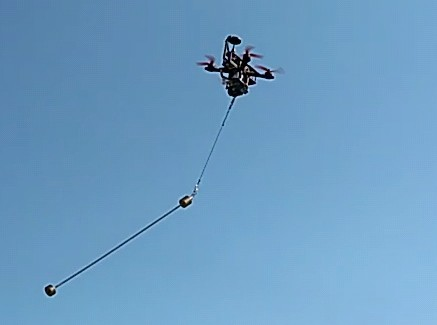
\includegraphics[width=0.6\linewidth]{practical_double_pendulum_2.jpg}
                \caption{Practical flight with an suspended elongated payload attached to Honeybee}
                \label{fig:practical_double_pendulum}
            \end{figure}     

            \paragraph
            One of the a prioir modelling assumptions mentioned in Section~\ref{sec:param_estimation},
            is that the suspended payload is a point mass.
            This reduced the considered suspended payload system to a simple pendulum in the white-box model.
            Figure~\ref{fig:practical_double_pendulum} shows a photo of an elongated payload 
            suspended from Honeybee during a practical flight
            This is a practical example of a dynamic payload 
            which deviates significantly from the point mass assumption.
            The mass distribution causes a relative rotation of the payload with respect to the suspended cable,
            which significantly affects the flight dynamics.

            \begin{figure}[htb]
    \centering
    \begin{tikzpicture}
        \begin{axis}[            
            xlabel = Time,
            ylabel = Payload angle,
            x unit = \si{\second},
            y unit = \si{\degree},
            xmin = 0,   xmax = 20,
            ymin = -20,  ymax = 25,
            grid = major,
            legend cell align = left,
            legend pos = north east,
            grid style = dashed,
            legend style = {font = \scriptsize},
            label style = {font = \scriptsize},
            tick label style = {font = \scriptsize},
            width = 0.95\columnwidth,
            height = 0.5\columnwidth,
            % initialize Dark2
            cycle list/Dark2,
            % combine it with 'mark list*':
            cycle multiindex* list = {
                Dark2\nextlist
            }
        ]
        
        \addplot+[mark = none, style = solid, ultra thick] 
        table[x = time, y = theta, col sep = comma] 
        {results/csv/step_predictions_Prac_2021-08-23_04_double_pend_m1_0.2_m2_0.1_l1-0.5_l2_0.62_wind-0.5.csv_dmd_201.csv};
        \addlegendentry{Measured}

        \addplot+[mark = none, style = dashed, ultra thick] 
        table[x = time, y = theta_hat, col sep = comma] 
        {results/csv/step_predictions_Prac_2021-08-23_04_double_pend_m1_0.2_m2_0.1_l1-0.5_l2_0.62_wind-0.5.csv_dmd_201.csv};
        \addlegendentry{DMD prediction}

        % \addplot+[mark = none, style = solid, ultra thick] 
        % table[x = time, y = theta, col sep = comma] 
        % {results/csv/step_predictions_Prac_2021-08-23_04_double_pend_m1_0.2_m2_0.1_l1-0.5_l2_0.62_wind-0.5.csv_dmd_201.csv};
        % \addlegendentry{White-box model}

        \end{axis}
    \end{tikzpicture} 
    
    \caption{Data-driven $\theta$ predictions of a double pendulum for a North velocity step input
        ($m_1 =$~\SI{0.2}{\kilo\gram}, $l_1 =$~\SI{0.5}{\meter}, $m_2 =$~\SI{0.1}{\kilo\gram}, $l_2 =$~\SI{0.6}{\meter})}
    \label{fig:prac_pediction_double_pend_theta_black}
\end{figure}


            \paragraph
            Figure~\ref{fig:prac_pediction_double_pend_theta_black} shows the measured and predicted payload angle
            of the practical dynamic payload.
            The irregular oscillations due to the double pendulum action of an elongated payload is clearly seen in the angle data.
            It appears that the prediction differs slightly from the measurement data at the peaks, 
            however this does not appear to be a significant error.
            Overall, it is clear that the \gls{DMDc} model captures the multi-frequency oscillations of the dynamic payload well.

            \begin{figure}[htb]
    \centering
    \begin{tikzpicture}
        \begin{axis}[            
            xlabel = Time,
            ylabel = Payload angle,
            x unit = \si{\second},
            y unit = \si{\degree},
            xmin = 0,   xmax = 20,
            ymin = -2.5,  ymax = 2.5,
            grid = major,
            legend cell align = left,
            legend pos = north east,
            grid style = dashed,
            legend style = {font = \scriptsize},
            label style = {font = \scriptsize},
            tick label style = {font = \scriptsize},
            width = 0.95\columnwidth,
            height = 0.5\columnwidth,
            % initialize Dark2
            cycle list/Dark2,
            % combine it with 'mark list*':
            cycle multiindex* list = {
                Dark2\nextlist
            }
        ]
        
        \addplot+[mark = none, style = solid, ultra thick] 
        table[x = time, y = vel, col sep = comma] 
        {results/csv/step_predictions_Prac_2021-08-23_04_double_pend_m1_0.2_m2_0.1_l1-0.5_l2_0.62_wind-0.5.csv_dmd_201.csv};
        \addlegendentry{Measured}

        \addplot+[mark = none, style = dashed, ultra thick] 
        table[x = time, y = vel_hat, col sep = comma] 
        {results/csv/step_predictions_Prac_2021-08-23_04_double_pend_m1_0.2_m2_0.1_l1-0.5_l2_0.62_wind-0.5.csv_dmd_201.csv};
        \addlegendentry{DMD prediction}

        % \addplot+[mark = none, style = solid, ultra thick] 
        % table[x = time, y = theta, col sep = comma] 
        % {results/csv/step_predictions_Prac_2021-08-23_04_double_pend_m1_0.2_m2_0.1_l1-0.5_l2_0.62_wind-0.5.csv_dmd_201.csv};
        % \addlegendentry{White-box model}

        \end{axis}
    \end{tikzpicture} 
    
    \caption{Data-driven $V_N$ model predictions of a double pendulum for a North velocity step input
        ($m_1 =$~\SI{0.2}{\kilo\gram}, $l_1 =$~\SI{0.5}{\meter}, $m_2 =$~\SI{0.1}{\kilo\gram}, $l_2 =$~\SI{0.6}{\meter})}
    \label{fig:prac_pediction_double_pend_theta_black}
\end{figure}

            
            \paragraph
            Figure~\ref{fig:prac_pediction_double_pend_vel_black} shows the measured and predicted velocity of the same flight.
            The superimposed frequencies are not as visible in the velocity oscillations as they were in the payload angle data.
            However these oscillations in the velocity response 
            still appear irregular compared to the simple payload data shown in Figure~\ref{fig:prac_pediction_single_pend_vel_black}.
            In Figure~\ref{fig:prac_pediction_double_pend_vel_black}, 
            the size of the velocity prediction deviates from the measurement data at the velocity overshoot.
            However, this error does not appear significant enough to affect the corresponding \gls{MPC} controller using this model.
            The shape of the velocity oscillations also appear to be captured well in the prediction.
            Recall that the prediction is propagated from an initial condition and the given input data only.
            The model does not use state measurements to readjust after the initial condition is taken.
            Therefore a accumulation in prediction error is expected as the prediction horizon increases.
            Because the model prediction matches the shape of the practical testing data so closely,
            it is expected that this model can be used for a practical \gls{MPC} implementation on practical data. 

            % As discussed in Chapter~\ref{chap:control_systems}, 
            % this prediction model can be used in an \gls{MPC} to optimise the control input to actively damp the payload swing angles.
            % It was also noted in Chapter~\ref{chap:control_systems} that the accuracy of the model 
            % has a direct impact on the performance of the controller.
            % Because the model prediction matches the practical testing data so closely,
            % it is expected that this model will 
            
   \section{HITL}

    \section{Conclusion}


